% $Header$
\documentclass{beamer}
\usepackage{tcolorbox}  %Cuadros de teoremas

% This file is a solution template for:

% - Giving a talk on some subject.
% - The talk is between 15min and 45min long.
% - Style is ornate.



% Copyright 2004 by Till Tantau <tantau@users.sourceforge.net>.
%
% In principle, this file can be redistributed and/or modified under
% the terms of the GNU Public License, version 2.
%
% However, this file is supposed to be a template to be modified
% for your own needs. For this reason, if you use this file as a
% template and not specifically distribute it as part of a another
% package/program, I grant the extra permission to freely copy and
% modify this file as you see fit and even to delete this copyright
% notice. 

\mode<presentation>{
  \usetheme{Warsaw}
%  % or ...
%
%  \setbeamercovered{transparent}
%  % or whatever (possibly just delete it)
}


\usepackage[spanish,es-tabla,es-nodecimaldot]{babel}
\usepackage{tikz}
\usepackage{pgf}  %Para realizar figures
\usepackage{xcolor} % Para los colores
\usepackage{enumerate}
\usepackage{graphicx}
\usepackage{array}

\title[ \hspace{21mm} \insertframenumber \ de \inserttotalframenumber ]
{Técnicas de conteo}

\subtitle
{Probabilidad, procesos aleatorios e inferencia} % (optional)

\author[] % (optional, use only with lots of authors)
{Ana Maritza Bello Yañez}
% - Use the \inst{?} command only if the authors have different
%   affiliation.

\institute[Instituto Politécnico Nacional] % (optional, but mostly needed)
{
  \inst{1}%
  Centro de Investigación en Computación
%  \and
%  \inst{2}%
%  Department of Theoretical Philosophy\\
%  University of Elsewhere
  }
% - Use the \inst command only if there are several affiliations.
% - Keep it simple, no one is interested in your street address.

\date[Short Occasion] % (optional)
{\today}

\keywords{conteo, permutación, combinación, variación, factorial}

\begin{document}

\begin{frame}
  \titlepage
\end{frame}

%\section*{Regla de multiplicación}
%\section*{Permutaciones}
%\section*{Combinaciones}
%\section*{Variaciones}
%\section*{Diagrama de árbol}

\begin{frame}{Regla de multiplicaci\'on}
  \onslide <1->
  \begin{block}{}
    Si queremos contar el número de formas en las que pueden ocurrir dos eventos
    simultáneos, podemos hacerlo usando la regla de la multiplicación.
  \end{block}
%\end{frame}
%
%
%\begin{frame}
  \onslide <2->
  \begin{block}{Regla}
    Si un evento puede ocurrir de $n_1$ formas diferentes, y para cada una de
    \'estas puede ocurrir un segundo evento simultaneo en $n_2$ formas diferentes, entonces los
    dos eventos pueden ocurrir de $n_1*n_2$ formas diferentes.
  \end{block}

  \onslide <2->
  Así, para una serie de $k$ eventos tenemos:

  \begin{block}{}
    \begin{equation}
      n_1*n_2*n_3*...*n_k
    \end{equation}
  \end{block}

  \onslide <3->
  Ejemplo:
  
  \begin{figure}
    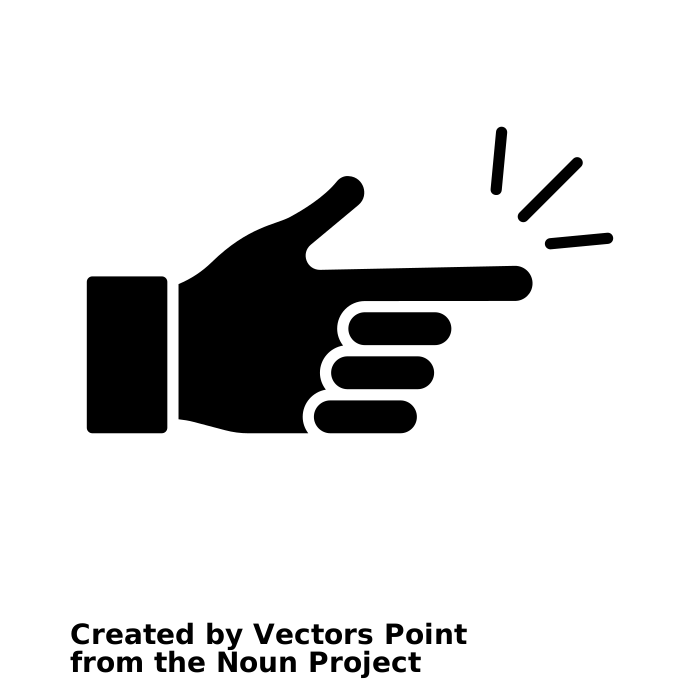
\includegraphics[width=2cm,angle=0,trim={1mm 170mm 1mm 250mm},clip]{figures/example-finger.png}
  \end{figure}

\end{frame}

\begin{frame}{Ejemplo de regla de multiplicaci\'on}
  \transdissolve
  \transblindshorizontal<3-4>
  \transwipe[duration=5]<5-6>

  \onslide <1->
  \begin{exampleblock}{}
    \begin{figure}
      \raggedleft
      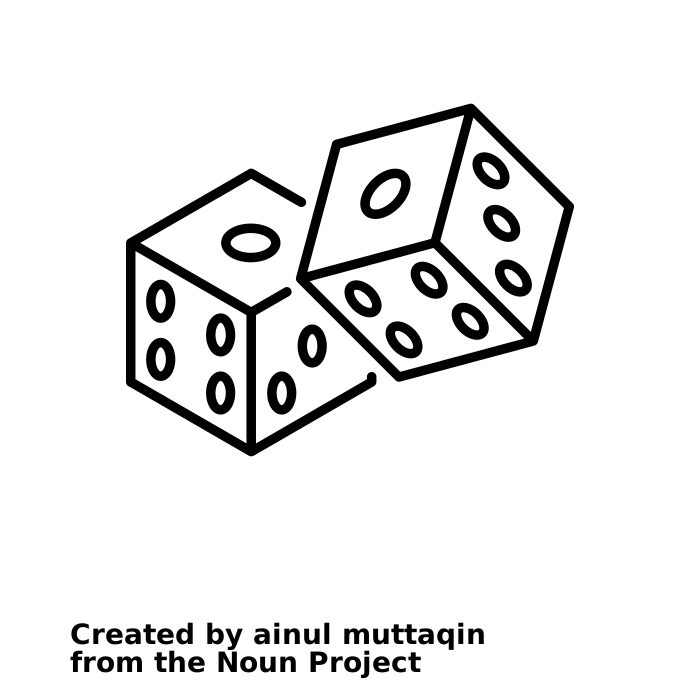
\includegraphics[width=2cm,angle=0,trim={1mm 210mm 1mm 200mm},clip]{figures/dice-roll.png}
    \end{figure}

    {¿De cuantas formas diferentes pueden caer dos dados \\
    de 6 caras si se lanzan al mismo tiempo?}
  \end{exampleblock}

    \vfill
    \onslide <2->{Soluci\'on:}
    \vfill
    \onslide <3->{El primer dado puede caer en cualquiera de $n_1 = 6$ maneras.}
    \vfill
    \onslide <4->{Para cada una de esas 6 maneras el segundo dado tambi\'en puede caer en $n_2 = 6$ formas.}
    \vfill
    \onslide <5->{Por lo tanto, el par de dados puede caer en $n_1*n_2 = (6)*(6) = 36$ formas posibles.}
  
\end{frame}

\begin{frame}{Diagrama de árbol}
  \begin{columns}
    \column{.5\textwidth}
      \begin{block}{}
        \begin{itemize}
          \onslide <1-> \item Los diagramas de árbol muestran todos los resultados posibles de un
          evento.
          \onslide <2-> \item Cada rama en un diagrama de árbol representa un posible resultado. 
          \onslide <3-> \item Los diagramas de árbol pueden usarse para encontrar el número de
          resultados posibles y calcular la probabilidad de los posibles resultados.
        \end{itemize}
      \end{block}

    \onslide <1->
    \column{.5\textwidth}
      \begin{figure}
        \centering
        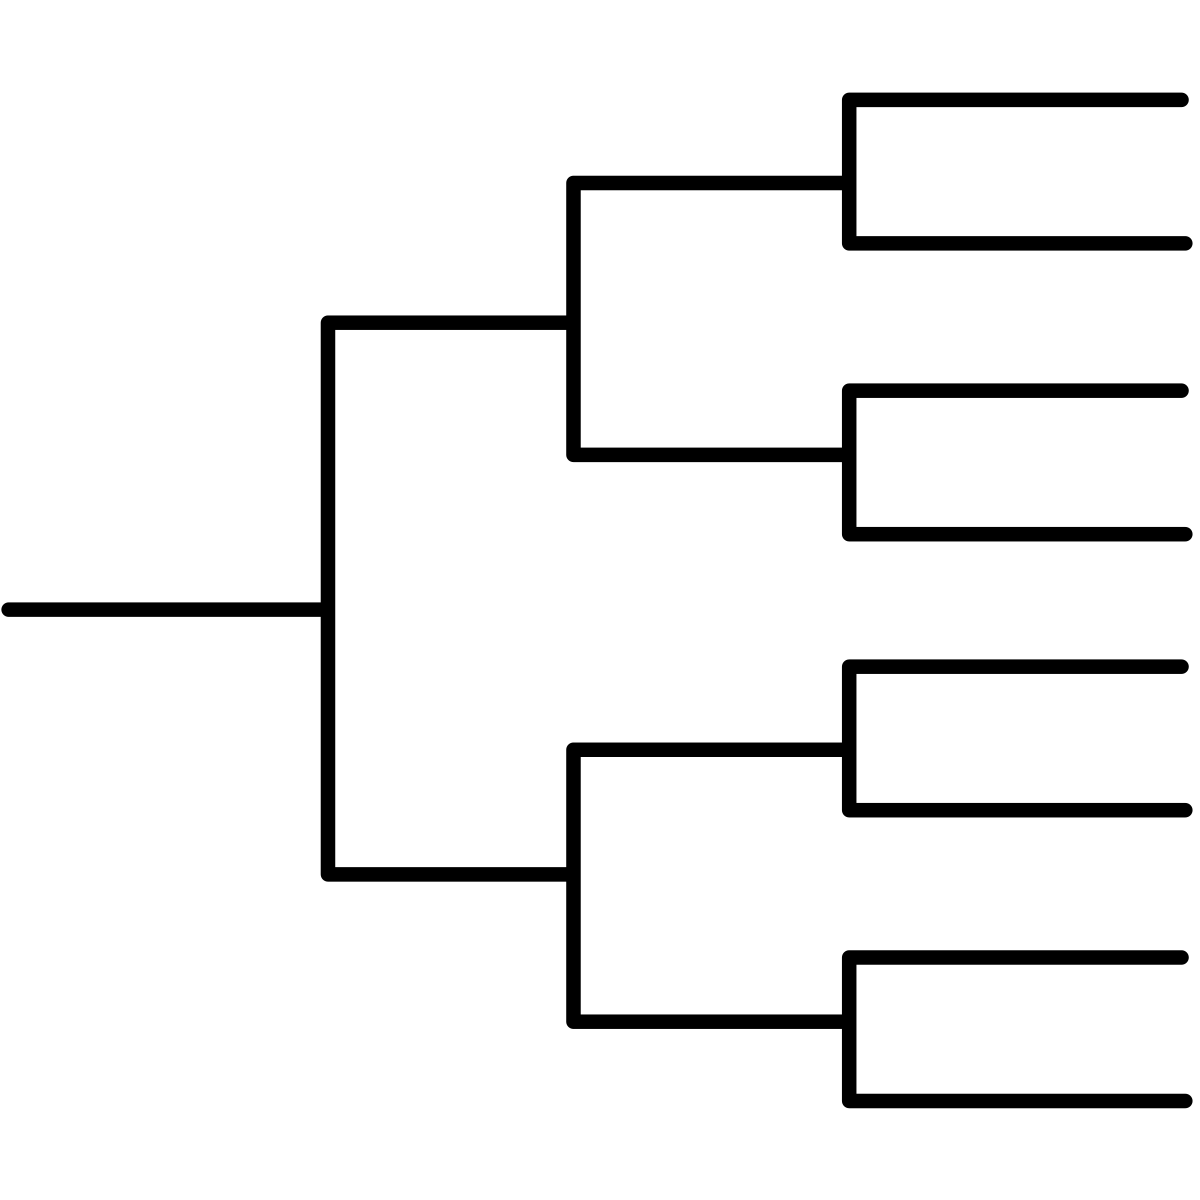
\includegraphics[width=3cm]{figures/tree.png}
      \end{figure}
  \end{columns}
\end{frame}

\begin{frame}{Ejemplo del diagrama de árbol}

  \begin{exampleblock}{Por ejemplo...}
    {Supongamos que vamos a comprar un helado. Entonces podemos escoger entre 3
    sabores, fresa (f), chocolate (ch) y limón(l). También, podemos escoger entre
    cono o vaso.}
  \end{exampleblock}

\end{frame}

\begin{frame}{Ejemplo del diagrama de árbol}
  %%%%%%%%%%%%%%%%%%%%%%%%%%%%%%%%%%%%%%%%%%%%%%%%%%%%%%%%%%%%%
  % Se pueden poner primero los conos y después los sabores?  %
  %%%%%%%%%%%%%%%%%%%%%%%%%%%%%%%%%%%%%%%%%%%%%%%%%%%%%%%%%%%%%
  \begin{figure}[h]
    \begin{center}		
    \begin{tikzpicture}[level distance=1cm, level 1/.style={sibling distance=3cm},
      level 2/.style={sibling distance=2cm}, every node/.style={circle, draw,
      align=center} ]
          \centering
          \node[circle,draw]{}
          child{
            node{f} child{
            node{c}} child{node{v}
          } 
          }
        child{
          node{ch} child{
          node{c}} child{node{v}
          }
        }
      child{
        node{v} child{
          node{c}} child{node{v}
          }
        };
        \end{tikzpicture}
      \end{center}
      \caption{Representación en el diagrama de árbol}
      \label{permutaciones_tree}
  \end{figure}
\end{frame}

\begin{frame}{Permutación, variación y combinación}

  \begin{block}{Definición}
    % DECIR QUE IMPORTA EL ORDEN
    \onslide <1->Las \textbf{permutaciones y combinaciones} son maneras de representar grupos de objetos
    al seleccionarlos de un conjunto y formar subconjuntos.
    \vfill
    \onslide <2-> Las \textbf{permutaciones} se refieren a la acción de ordenar u organizar los miembros de
    un conjunto en algún tipo de orden o secuencia. Si un conjunto está ordenado, el
    proceso de reodenar sus elementos se llama permutar.
    \vfill
    \onslide <3-> La \textbf{variación} es la disposición de una parte del total de los elementos en un
    orden determinado.
    \vfill
    \onslide <4-> A diferencia de las permutaciones y variaciones, en la \textbf{combinación} no importa el orden de la
    selección de los subconjuntos.

  \end{block}

\end{frame}

\begin{frame}{Permutación, variación y combinación}

  \begin{tabular}{lcc}
    \onslide <1-> & ¿Importa el orden?  & ¿Entran todos los elementos? \\
    \onslide <2-> Permutación & Si                  &   Si    \\
    \onslide <3-> Variación   & Si                  &   No    \\
    \onslide <4-> Combinación & No                  &   No
  \end{tabular}

\end{frame}

\begin{frame}{Teorema de permutaciones}

  \onslide<1->
  \begin{block}{Definición}
    El total de permutaciones de $n$ objetos distintos tomados de $r$ formas a la
    vez está dado por:
    \begin{equation}
        P(n,r) =  \frac{n !}{(n - r)!}
    \end{equation}
  \end{block}
  \onslide<2->

  Ejemplo:
  
  \begin{figure}
    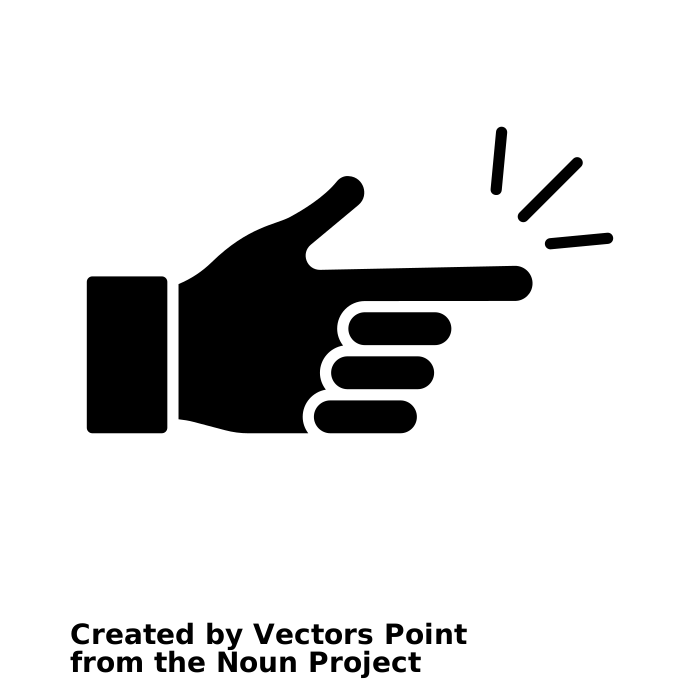
\includegraphics[width=2cm,angle=0,trim={1mm 216mm 1mm 200mm},clip]{figures/example-finger.png}
  \end{figure}

\end{frame}

\begin{frame}{Ejemplo de permutación} 
  % Problema de monti hol? 
  % Problema del cumpleaños  
  \onslide<1->
  \begin{exampleblock}{Ejemplo}
    Encuentre el número de permutaciones del conjunto de letras $A =
    \{a,b,c,d,e,f\}$, tomando 3 al mismo tiempo y sin que se repitan. Es decir,
    ¿Cuantas palabras de 3 letras podemos formar a partir de las 6 anteriores?
  \end{exampleblock}
  
  \onslide<2->
  Solución:

  \begin{itemize}
    \item La primera letra podemos escogerla de 6 maneras diferentes.
    \onslide<3->\item La segunda letra podemos escogerla de 5 maneras diferentes.
    \onslide<4->\item La tercera letra podemos escogerla de 4 maneras diferentes.
  \end{itemize}
  De acuerdo a la regla de la multiplicación tenemos:
  \begin{exampleblock}{}
    \centering
    $6*5*4 = 120$
  \end{exampleblock}

\end{frame}

\begin{frame}{Ejemplo de permutación}
  También podemos sustituir en la fórmula y el resultado será el mismo:
  \begin{exampleblock}{}
    \begin{equation}
        P(n,r) =  \frac{6 !}{(6 - 3)!} = \frac{720}{6} = 120
    \end{equation}
  \end{exampleblock}
\end{frame}

\begin{frame}{Permutación con reemplazo y sin reemplazo}
  \onslide<1->
  \begin{exampleblock}{Ejemplo}
    \begin{figure}
      \raggedleft
      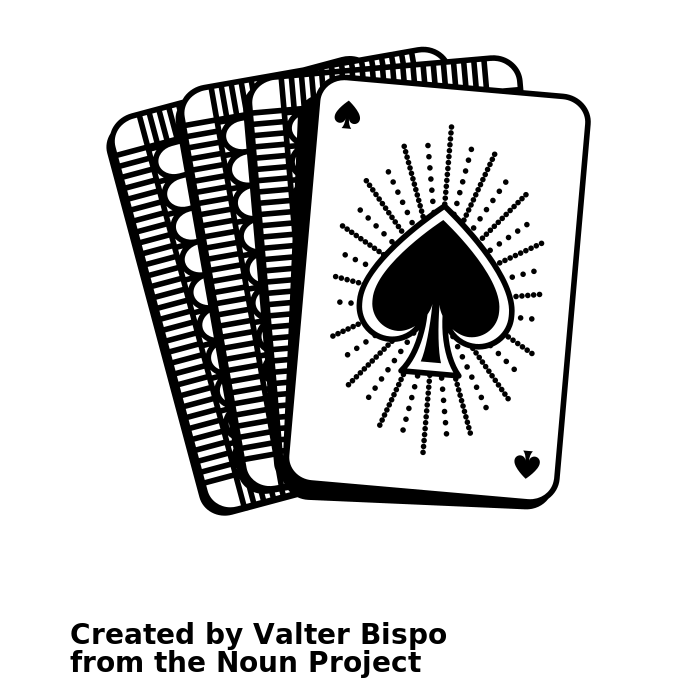
\includegraphics[width=2cm,angle=0,trim={1mm 250mm 1mm 310mm},clip]{figures/deck-of-cards.png}
    \end{figure}

    ¿De cuantas maneras posibles se pueden escoger 3 
    \\cartas de una baraja de 52
    cartas?
    \begin{itemize}
      \item Si hay reemplazo (la carta se regresa al mazo)
      \item Si no hay reemplazo (la carta no se regresa al mazo)
    \end{itemize}
  \end{exampleblock}

  \onslide<2->
  \begin{exampleblock}{Con reemplazo}
    \centering
    $52*52*52 = 52^{3} = 140 608$
  \end{exampleblock}

  \onslide<2->
  \begin{exampleblock}{Sin reemplazo}
    \centering
    $52*51*50 = 132,600$
  \end{exampleblock}

\end{frame}

\begin{frame}{Permutación}

  \textbf{Definición}


  Una \textbf{permutaci\'on} de un conjunto o lista es un arreglo de dichos
  elementos en alg\'un orden sin repeticiones ni omisiones.

\end{frame}

\begin{frame}{Permutación}
  Considerando la lista de números
  \begin{equation}
    A = {1,2,3}
  \end{equation}

  Tenemos 6 arreglos distintos que podemos calcular con la regla de
  multiplicación.
    
  Hay 
  \vfill
  $n_1 = 3$ opciones para la primera posición, 
  \vfill
  $n_2 = 2$ para la segunda posición y para la última opción hay 
  \vfill
  $n_3 = 1$ opción.

\end{frame}

\begin{frame}{Permutación}
  Entonces tenemos $n_1 * n_2 * n_3 = 6$ permutaciones.
  \vfill
  Por lo que $n$ objetos distintos se pueden arreglar en
  $n(n-1)(n-2)...(3)(2)(1)$ formas.
  \vfill
  Con lo anterior podemos decir que para cualquier entero no negativo $n,n!$
  denominado "$n$ factorial"se define como:
  \vfill
  $N! = n(n-1)...(2)(1)$
  \vfill
  Con el caso especial de cero, que está dado por:
  $0!=1$
\end{frame}


\begin{frame}{Permutación}
\textbf{Teorema}
\vfill
El número de permutaciones de $n$ objetos es $n!$.

\end{frame}


\begin{frame}{Paridad de una permutación}
La paridad o signatura de una permutación vale 1 si esta es par y -1 si es
impar.
\vfill
Sea una permutación $\sigma$. La definición de la signatura de $\sigma$ se hace contando las inversiones.

\vfill

Sean $i < j$ dos elementos distintos comprendidos entre $1$ y $n$. Se dice que
se tiene una inversión del par ${i, j}$ para $\sigma$ cuando $\sigma(i) > \sigma(j)$. 
\vfill
Se dice que una permutación es par cuando presenta un número par de inversiones.
\vfill
Se dice impar cuando la cantidad de inversiones es impar.

\end{frame}


\begin{frame}{Ejemplo de paridad de una permutación}
  Sea una lista de elementos $A={1,2,3}$
  \vfill
  Permutación par $A'={2,3,1}$
  \vfill
  Permutación impar $A''={3,2,1}$
  \vfill
  ¿Como saber si la permutación es par o impar?
\end{frame}

\begin{frame}{Ejemplo de paridad de una permutación}

  Para la permutación par $A'={2,3,1}$ calculamos las inversiones.
  \vfill
  Tomamos todos los pares $i,j$ del conjunto que cumplan la condición $i < j$.
  \vfill
  Para $i=(1)$ y $j=(2,3)$
  
  \vfill
  $(1,2)$ Tenemos $\sigma(1)=2$ y $\sigma(2)=3$ Por lo que $\sigma(1) < \sigma(2)$ \\
  $(1,3)$ Tenemos $\sigma(1)=2$ y $\sigma(3)=1$ Por lo que $\sigma(1) > \sigma(3)$
  \vfill
  
  La inversión cumple que $\sigma(i) > \sigma(j)$.
  
  \vfill
  
  Para $i=(2)$ y $j=(3)$
  \vfill
  $(2,3)$ Tenemos $\sigma(2)=3$ y $\sigma(3)=1$ Por lo que $\sigma(2) > \sigma(3)$\\
  Es inversión
  \vfill
  Total de inversiones = 2

\end{frame}


\begin{frame}{Ejemplo de paridad de una permutación}

  Para la permutación impar $A'={3,2,1}$ calculamos las inversiones.
  \vfill
  Tomamos todos los pares $i,j$ del conjunto que cumplan la condición $i < j$.
  \vfill
  Para $i=(1)$ y $j=(2,3)$
  
  \vfill
  $(1,2)$ Tenemos $\sigma(1)=3$ y $\sigma(2)=2$ Por lo que $\sigma(1) > \sigma(2)$ \\
  $(1,3)$ Tenemos $\sigma(1)=3$ y $\sigma(3)=1$ Por lo que $\sigma(1) > \sigma(3)$
  \vfill
  
  Son inversiones porque cumplen que $\sigma(i) > \sigma(j)$.
  
  \vfill
  
  Para $i=(2)$ y $j=(3)$
  \vfill
  $(2,3)$ Tenemos $\sigma(2)=2$ y $\sigma(3)=1$ Por lo que $\sigma(2) > \sigma(3)$\\
  También es inversión
  \vfill
  Total de inversiones = 3

\end{frame}


\end{document}


